\documentclass{article}\usepackage[]{graphicx}\usepackage[]{color}
%% maxwidth is the original width if it is less than linewidth
%% otherwise use linewidth (to make sure the graphics do not exceed the margin)
\makeatletter
\def\maxwidth{ %
  \ifdim\Gin@nat@width>\linewidth
    \linewidth
  \else
    \Gin@nat@width
  \fi
}
\makeatother

\definecolor{fgcolor}{rgb}{0.345, 0.345, 0.345}
\newcommand{\hlnum}[1]{\textcolor[rgb]{0.686,0.059,0.569}{#1}}%
\newcommand{\hlstr}[1]{\textcolor[rgb]{0.192,0.494,0.8}{#1}}%
\newcommand{\hlcom}[1]{\textcolor[rgb]{0.678,0.584,0.686}{\textit{#1}}}%
\newcommand{\hlopt}[1]{\textcolor[rgb]{0,0,0}{#1}}%
\newcommand{\hlstd}[1]{\textcolor[rgb]{0.345,0.345,0.345}{#1}}%
\newcommand{\hlkwa}[1]{\textcolor[rgb]{0.161,0.373,0.58}{\textbf{#1}}}%
\newcommand{\hlkwb}[1]{\textcolor[rgb]{0.69,0.353,0.396}{#1}}%
\newcommand{\hlkwc}[1]{\textcolor[rgb]{0.333,0.667,0.333}{#1}}%
\newcommand{\hlkwd}[1]{\textcolor[rgb]{0.737,0.353,0.396}{\textbf{#1}}}%

\usepackage{framed}
\makeatletter
\newenvironment{kframe}{%
 \def\at@end@of@kframe{}%
 \ifinner\ifhmode%
  \def\at@end@of@kframe{\end{minipage}}%
  \begin{minipage}{\columnwidth}%
 \fi\fi%
 \def\FrameCommand##1{\hskip\@totalleftmargin \hskip-\fboxsep
 \colorbox{shadecolor}{##1}\hskip-\fboxsep
     % There is no \\@totalrightmargin, so:
     \hskip-\linewidth \hskip-\@totalleftmargin \hskip\columnwidth}%
 \MakeFramed {\advance\hsize-\width
   \@totalleftmargin\z@ \linewidth\hsize
   \@setminipage}}%
 {\par\unskip\endMakeFramed%
 \at@end@of@kframe}
\makeatother

\definecolor{shadecolor}{rgb}{.97, .97, .97}
\definecolor{messagecolor}{rgb}{0, 0, 0}
\definecolor{warningcolor}{rgb}{1, 0, 1}
\definecolor{errorcolor}{rgb}{1, 0, 0}
\newenvironment{knitrout}{}{} % an empty environment to be redefined in TeX

\usepackage{alltt}

\usepackage{natbib}
\usepackage{geometry}
\geometry{verbose,tmargin=3cm,bmargin=3cm,lmargin=3cm,rmargin=3cm}
\usepackage{verbatim}
\usepackage{authblk}
\usepackage{setspace}
\usepackage[margin=10pt,font=small,labelfont=bf]{caption}
\usepackage{hyperref}
\usepackage{float}
\usepackage{indentfirst}

\doublespacing

\title{NUCOMBog: A R package to run the NUCOM-Bog model and process its outputs}
\author[1,2]{J.W.M. Pullens\thanks{corresponding author, jeroenpullens@gmail.com, executable of the model is available on request at corresponding author}}
\author[3]{M. Bagnara}
\author[3]{F. Hartig}
\affil[1]{Department of Sustainable Agro-ecosystems and Bioresources, Research and Innovation Centre, Fondazione Edmund Mach (FEM), Via E. Mach 1, 38010 San Michele all'Adige, Italy}
\affil[2]{Hydromet, Department of Civil and Environmental Engineering and Environmental Research Institute, University College Cork, Cork, Ireland}
\affil[3]{University of Freiburg, Germany}
\date{}
\IfFileExists{upquote.sty}{\usepackage{upquote}}{}
\begin{document}
\maketitle

\section{Abstract}
The model NUCOM-Bog (NUtrient cycling and COMpetition) describes the vegetation, carbon, nitrogen and water dynamics of peatland ecosystems \citep{Heijmans2008a}. This model is derived from earlier NUCOM models \citep{Berendse1988,Oene1999}. The NUCOMBog package links the model, which is written in Delphi, to the R infrastructure. It runs on a monthly time step and the competition is based on light and nitrogen. For more details about NUCOM-Bog, see \cite{Heijmans2008a}. The executable of the model is available on request at the corresponding author.

\section{Model}
\begin{figure*}[htb]
\centering
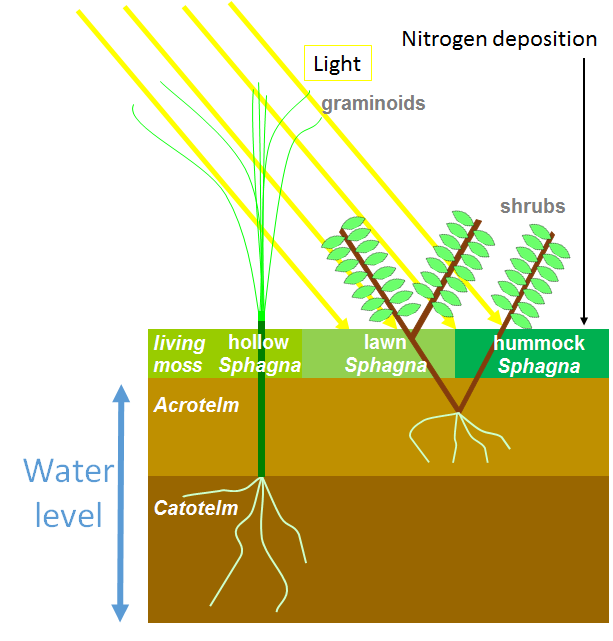
\includegraphics[width=10 cm]{figure1}
\caption{Schematic representation of the NUCOMBog model with five plant functional types, adapted from \citet{Heijmans2008a}.}
\label{figure: model}
\end{figure*}
NUCOMBog simulates the dynamics of five plant function types (PFTs): graminoids, ericaceous shrubs and three groups of \emph{Sphagnum} mosses, lawn, hollow and hummock mosses. The PFTs compete for light and nitrogen, where the light is first available for the taller graminoids, then the shrubs and finally the mosses (see Fig.~\ref{figure: model}). Each time step (one month) NUCOMBog calculates the potential growth rate (Gpot) based on the amount of intercepted light (LI), maximum growth rate (Gmax), the ${CO_2}$ concentration, air temperature (temp) and water table depth (WTD). 
\begin{equation} \label{eq1}
Gpot = LI * Gmax * f(CO2) * f(temp) * f(WTD)
\end{equation}
Each plant functional type has its own optimal range for temperature and water level depth. The potential growth rate is then further restricted by the amount of nitrogen available. The model calculates the water table depth (WTD) based on precipitation, potential evapotranspiration (calculate from \cite{Penman1946}) and drainage. The drainage in the model is a very basic process, it represents surface run-off and lateral outflow through the living moss layer \citep{Heijmans2008a}.
\\ The nitrogen from wet and dry atmospheric deposition is first available for the mosses \citep{Heijmans2002}. The excess nitrogen leaches into the soil, where it is available for the ericaceous shrubs with their shallow roots. Deeper in the soil the nitrogen is available for the roots of the graminoids. The same pattern holds for the dead organic matter (DOM). The DOM is incorporated in the moss layer, before it enters the top soil called "acrotelm". In this layer the water table depth fluctuates, so both anaerobic and aerobic decomposition takes place. The permanent waterlogged soil is called "catotelm", the lack of oxygen makes the decomposition rates lower compared to the acrotelm (see Fig.~\ref{figure: model}). The model calculates the boundary between acrotelm and catotelm as the yearly deepest mean water level. The depth of the acrotelm and the catotelm is being calculated based on the amount of carbon present and the bulk density of the source of the carbon. When the carbon sequestration is bigger than the decomposition the complete peat layer can increase in depth, when the peatland is losing carbon the peat layer can decrease in depth in the same manner.
\\ In the model all PFTs are given a minimum cover of 0.1\%, by doing so the PFT has a starting biomass, when the growing conditions are becoming optimal (comparable with a permanent seed bank). With this starting biomass the PFT is able to establish and start competing for light and nitrogen.

The NUCOM-Bog model \citep{Heijmans2008a} calculates the monthly net primary production (NPP). For this package, NUCOM-Bog has been modified in such a way that is also outputs the monthly heterotrophic respiration. In this case the net ecosystem exchange (NEE) can be calculated:
\begin{equation} \label{eq2}
NEE = NPP - heterotrophic\ respiration
\end{equation}

In this package, the NEE follows the micro-meteorological sign convention, i.e. a negative NEE is an carbon uptake for the ecosystem. All fluxes are in gram carbon per square meter per month (gC m\textsuperscript{2} month\textsuperscript{1}).

The model calculates the water table depth (WTD) based on precipitation, potential evapotranspiration and drainage. The drainage in the model is a very basic process, drainage represents surface run-off and lateral outflow through the living moss layer \citep{Heijmans2008a}. The model gives water table depth (WTD) in meters and negative values indicate water table depths below ground surface.

The model needs three types of input data, all which need to be in the input folder as a ".txt" file.
An example of the structure of the folder and the data of the example can be downloaded from \url{https://github.com/jeroenpullens/NUCOMBog_data}. The data used in this publication are from \cite{Heijmans2008a}. The tree inputs are:

\paragraph{Initial values}
The model needs to be initialized with biomass values, preferable from field measurements. In the model the biomass of the vascular plants is separated in "organs" (leaf, shoot, root), while the biomass of the mosses is only the mass of the "shoot". The biomass needs to be separated into grams of carbon and grams of nitrogen per plant organ. Also the carbon and nitrogen of each specific plant organ stored/sequestrated in the acrotelm and catotelm is needed. As well as an initial water table depth and average water table depth.

\paragraph{Environmental data}
The environmental data should contain the yearly atmospheric ${CO_2}$ concentration in ppm and nitrogen deposition (both wet and dry) in kg N per hectare.

\paragraph{Climatic data}
The climatic data should contain monthly temperature, precipitation, and potential evapotranspiration. NUCOM-Bog was designed to run with the calculated Penman potential evapotranspiration \citep{Penman1946}.

\section{The NUCOMBog R package}
The NUCOMBog R package provides several functions to setup and run the model.

\subsection*{setupNUCOM} \label{ssec:setupNUCOM}
In order to run the model a setup structure needs to be made. In this way the model knows the working directory, the climatic, environmental data, the initial biomass values, the start year and the end year. The model starts in January of the start year and ends in December of the end year. In the setup also the output is specified, see section: \nameref{ssec:getData}. For both the single core run and the multi-core run the same setup function can be used. This can be done by setting the parameter "parallel" to TRUE or FALSE, the default value is FALSE. "Separate" can only be use in parallel, it can be used to run the model with a list of parameters where all parameters are run individually, in contrast to a complete parameter list. Parameters for which no value has been given these parameters are set to the original value, see \nameref{ssec:runNUCOM}.

In some runs a spin-up period is used. During this spin-up the model can reach a stable equilibrium, this can be useful when the initial biomass values are not completely known. Since the data from not spin-up is not always needed for analysis, these values can be neglected by R. In the setup function the parameter "Startval" is implemented for that reason. The "Startval" has to be the row number of the output, i.e. if the model was run from 1970-2005 and only the data from January 2000 onward is needed. The start value has to be set to (2000-1970)*12 = 360. This "Startvalue" will be used in the getData function.

\subsection*{getData} \label{ssec:getData}
The getData function retrieves the monthly data from the model run. The data of monthly output file is loaded into the global environment.
The output that can be retrieved is Net Primary Production ("NPP"), Heterotrophic respiration ("hetero\textunderscore resp"), Net Ecosystem Exchange ("NEE") and water table depth ("WTD"). The "Startvalue" can also be set, the "Startval" has to be the row number of the output, i.e. if the model was run from 1970-2005 and only the data from January 2000 onward is needed. The start value has to be set to (2000-1970)*12 = 360.

\subsection*{runNUCOM} \label{ssec:runNUCOM}
When the setupNUCOM function has run, the setup is used to run the model. The presented function here only runs on a single core, for the multi-core run, see \nameref{ssec:runparallelNUCOM}. To run NUCOMBog we need the setup as previously described and potentially the parameter values. The parameter values need to be in a data frame format with two columns. The column names have to be "names" and "values", both without capital letter. When no parameters or few parameters are given to the model, the model uses the values provided by \cite{Heijmans2008a} for the parameters which are not provided. The names are the same as in the paper, but to identify to which PFT the variable corresponds, the first four letters are used, so eric, gram, humm, lawn and holl. For example the maximum potential growth rate of the graminoids is gram\textunderscore maxgr. The shrubs are defined ericaceous, e.g. the maximum potential growth rate is eric\textunderscore maxgr.

During the run the parameter file is created in the input folder. In the output folder the monthly and yearly output files are created. Example input files and the folder structure can be downloaded from \url{https://github.com/jeroenpullens/NUCOMBog_data}.

\subsection*{runparallelNUCOM} \label{ssec:runparallelNUCOM}
This function is used to run the model over multiple cores, this is particularly useful when multiple parameter sets need to be run. This function makes use of the snowfall \citep{Knaus2013} package. To run the model in parallel, the type of cluster is needed, by default this is set to "SOCK". The model has not been tested on other cluster types so far. In the runparallelNUCOM function also the amount of cores, that are available for the computation, are needed. By default it is set to "1".

During the parallel run of the model for each provided parameter set a new folder is created in which the files with the climatic, environmental and initial data and the executable is copied. This has the advantage that the parameter files and the output files are in one folder, so no specific tracking in the cluster is needed.

The created folders are also very small (smaller than 2 MB) and therefore disk space issues are most likely not occurring.

\section{Example Lille Vildmose, Denmark}
In this section we will present an example of NUCOMBog. For this run the data from the Lille Vildmose, Denmark as presented in \cite{Heijmans2008a} is used. The data can be downloaded from \url{https://github.com/jeroenpullens/NUCOMBog_data}.



\begin{knitrout}
\definecolor{shadecolor}{rgb}{0.969, 0.969, 0.969}\color{fgcolor}\begin{kframe}
\begin{alltt}
\hlstd{test_setup_singlecore} \hlkwb{<-} \hlkwd{setupNUCOM}\hlstd{(}\hlkwc{mainDir} \hlstd{=} \hlstr{"/home/jeroen/MEE_model/"}\hlstd{,}
    \hlkwc{climate} \hlstd{=} \hlstr{"ClimLVMhis.txt"}\hlstd{,} \hlkwc{environment} \hlstd{=} \hlstr{"EnvLVMhis.txt"}\hlstd{,}
    \hlkwc{inival} \hlstd{=} \hlstr{"inivalLVMhis.txt"}\hlstd{,} \hlkwc{start} \hlstd{=} \hlnum{1766}\hlstd{,} \hlkwc{end} \hlstd{=} \hlnum{1999}\hlstd{,} \hlkwc{type} \hlstd{=} \hlkwd{c}\hlstd{(}\hlstr{"NEE"}\hlstd{,}
        \hlstr{"WTD"}\hlstd{,} \hlstr{"NPP"}\hlstd{,} \hlstr{"hetero_resp"}\hlstd{),} \hlkwc{parallel} \hlstd{= F)}
\hlstd{output} \hlkwb{<-} \hlkwd{runNUCOM}\hlstd{(}\hlkwc{setup} \hlstd{= test_setup_singlecore,} \hlkwc{parameters} \hlstd{=} \hlkwa{NULL}\hlstd{)}
\end{alltt}
\end{kframe}
\end{knitrout}

What we can see here is that the model has been run without any given parameters and therefore the integrated values from \cite{Heijmans2008a} are used. The model was run from January 1766 till December 1999. The net primary production, net ecosystem exchange and water table depth are plotted from 1980 till 1999 (Figure \ref{fig:plot_output}).

\begin{knitrout}
\definecolor{shadecolor}{rgb}{0.969, 0.969, 0.969}\color{fgcolor}\begin{figure}[H]

{\centering 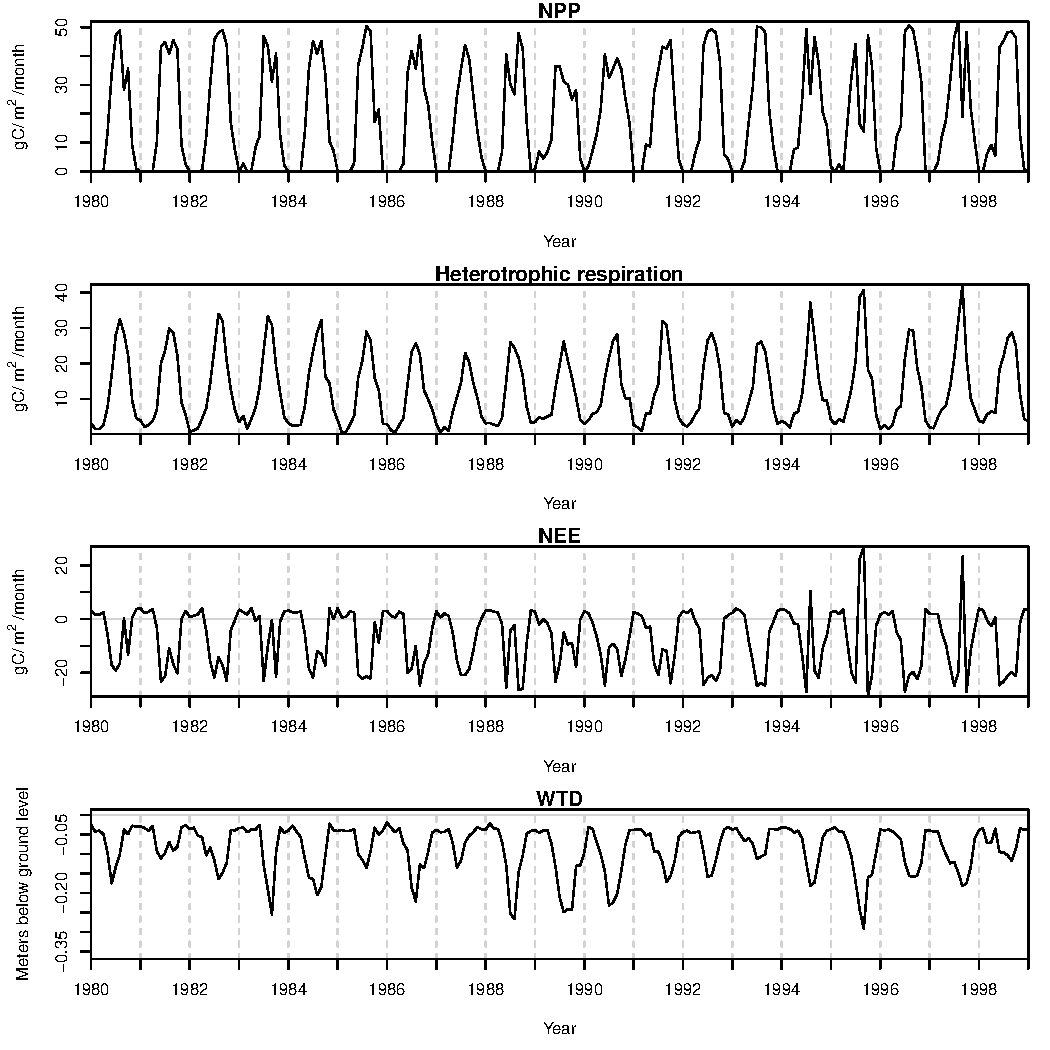
\includegraphics[width=\maxwidth]{figure/plot_output-1} 

}

\caption[Simulated monthly NPP, NEE, heterotrophic respiration and WTD from 1980 till 1999]{Simulated monthly NPP, NEE, heterotrophic respiration and WTD from 1980 till 1999.}\label{fig:plot_output}
\end{figure}


\end{knitrout}

The seasonal dynamics can be seen in the plot of the NPP, NEE and heterotrophic respiration, in which the greatest uptake takes place during the summer months. During some of the summer months the NEE 'peaks' close to zero or even above zero, these episodes match with a drop in water table depth. This could indicate that the plants were water stressed. During the winters the NEE is bigger than 0 gC m\textsuperscript{2} month\textsuperscript{1}, indicating a loss of carbon, through heterotrophic respiration.

\begin{knitrout}
\definecolor{shadecolor}{rgb}{0.969, 0.969, 0.969}\color{fgcolor}\begin{figure}[H]

{\centering 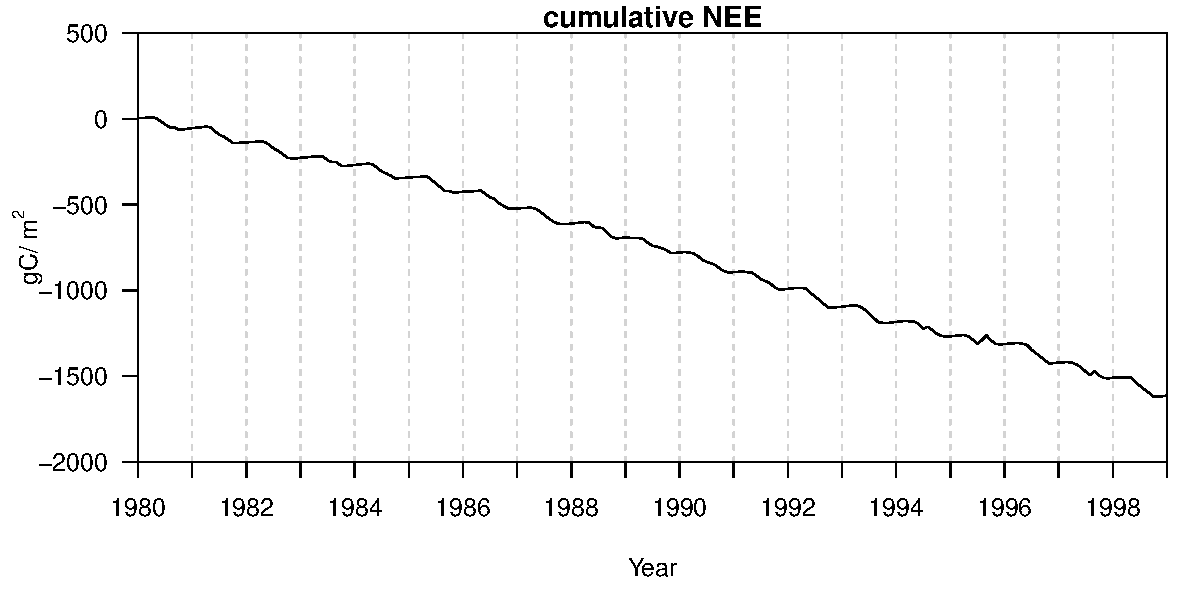
\includegraphics[width=\maxwidth]{figure/plot_cumsum-1} 

}

\caption[Cumulative monthly net ecosystem exchange from 1980 until 1999]{Cumulative monthly net ecosystem exchange from 1980 until 1999.}\label{fig:plot_cumsum}
\end{figure}


\end{knitrout}

When we plot the cumulative modeled NEE, we see that the modeled Lil Vildmose site is acting as a carbon sink, i.e. sequestering carbon, see Figure \ref{fig:plot_cumsum} .

\begin{knitrout}
\definecolor{shadecolor}{rgb}{0.969, 0.969, 0.969}\color{fgcolor}\begin{figure}[H]

{\centering 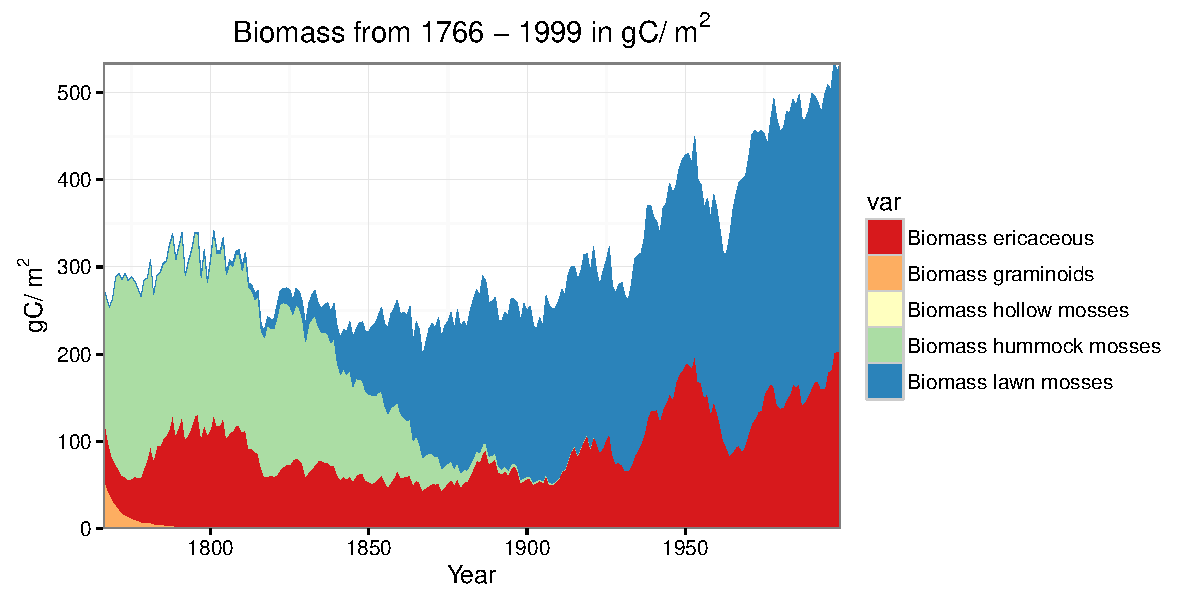
\includegraphics[width=\maxwidth]{figure/plotbiomass-1} 

}

\caption[Biomass composition of the five different PFTs from 1766 till 1999]{Biomass composition of the five different PFTs from 1766 till 1999.}\label{fig:plotbiomass}
\end{figure}


\end{knitrout}

Figure \ref{fig:plotbiomass} indicates that the initial biomass of the graminoids was set too high. The plants die within 40 years and never return. At this location there is no hollow moss present and the initial values were therefore set to 0 gC m\textsuperscript{2}. The last 100 years the  vegetation composition is stabilizing, only ericaceous shrub species and lawn mosses are present. Both PFTs are increasing their biomass over time, due to ${CO_2}$ fertilization and an increase in temperature.



\section{Acknowledgements}
The authors would like to thank Ramiro Silveyra Gonzalez for his help with the development for this package. The authors would also like to thank Monique Heijmans for providing the NUCOM-Bog model. This work was supported by a STSM grant to JWMP from COST Action FP1304 (Profound) \url{http://cost-profound.eu/site/}.

\bibliographystyle{apalike}
\bibliography{library}

\end{document}
